\section{Malware Metadata Study}
\label{sec:meta}

This section presents our study of VirusTotal malwares’ metadata. 
This part of our study is performed in 4 dimensions:

{\bf What?} What is file size distributions of malwares on VirusTotal? 
How many malwares are 32-bit, and how many malwares are 64-bit? 

\begin{figure}[t!]
\begin{center}
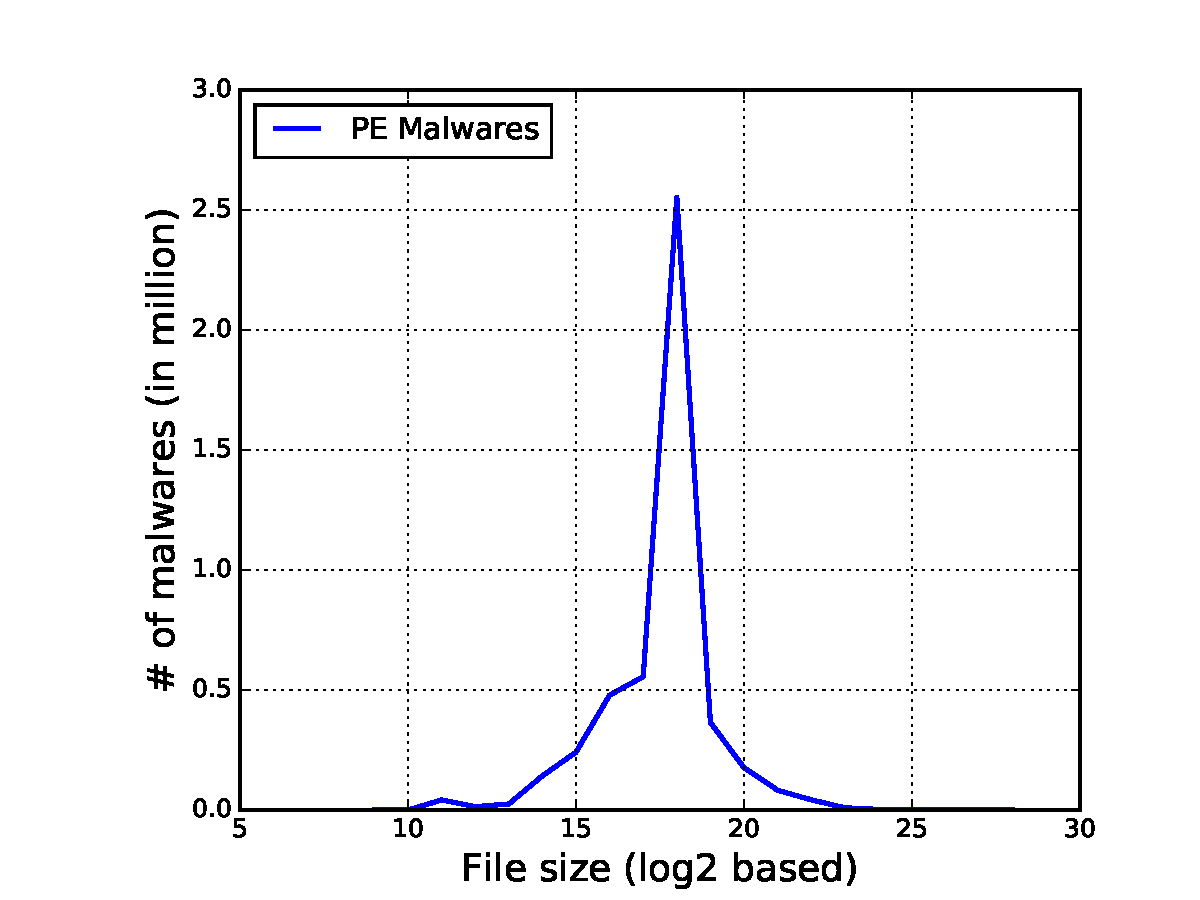
\includegraphics[width=2.5in]{figure/size}
\mycaption{fig:size}{Size distribution for malwares on VirusTotal in November 2015.}
{The number of malwares falling into each log2-based size category in November 2015.}
%\label{fig:new}
\end{center}
%\vspace{-0.3in}
\end{figure}

Figure~\ref{fig:size} shows the size distribution for malwares. 
The smallest malware is only 704 bytes, and the largest one is more than 502 MB. 
95.3\% of malwares fall into the range from 16 KB to 2 MB. 

VirusTotal does not provide tags to differ 64-bit malwares from 32-bit malwares directly. 
We sample 10000 malwares and download their executable binaries from VirusTotal.
We apply Linux command file to each sampled malware binary. 
64-bit malwares are labeled with PE32+ by file command. 
In total, there are only 127 64-bit malwares in our sampled set. 

{\bf Who?} How many real-world users submit malwares on VirusTotal? 
How malware submissions distribute among different users? 

\begin{figure}[t!]
\begin{center}
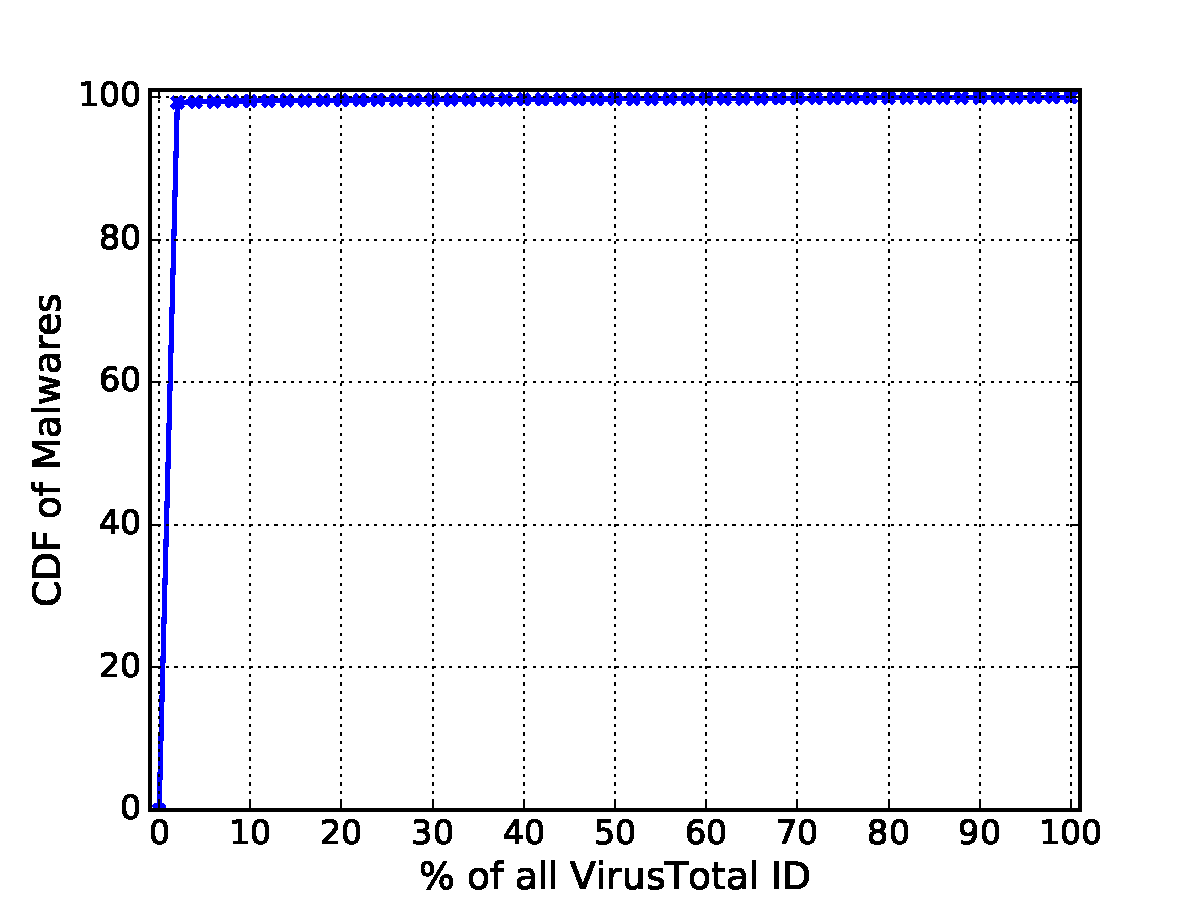
\includegraphics[width=2.5in]{figure/id}
\mycaption{fig:id}{Skewness of malware submissions from different users in November 2015.}
{Accumulation distribution of malwares submitted by different users in November 2015.}
%\label{fig:acum}
\end{center}
\vspace{-0.25in}
\end{figure}

For around 0.6 million malwares, VirusTotal fails to provide their submission IDs. 
The left 4 million malwares are submitted by 20739 distinct users.
As shown in Figure~\ref{fig:id}, malware submissions are distributed unbalanced among different users.
15748 users only submit one malware. 
The user, with largest submission number, submitted more than 3 million malwares. 

{\bf Where?} Where do malware submissions come from? 

\begin{figure}[t!]
\begin{center}
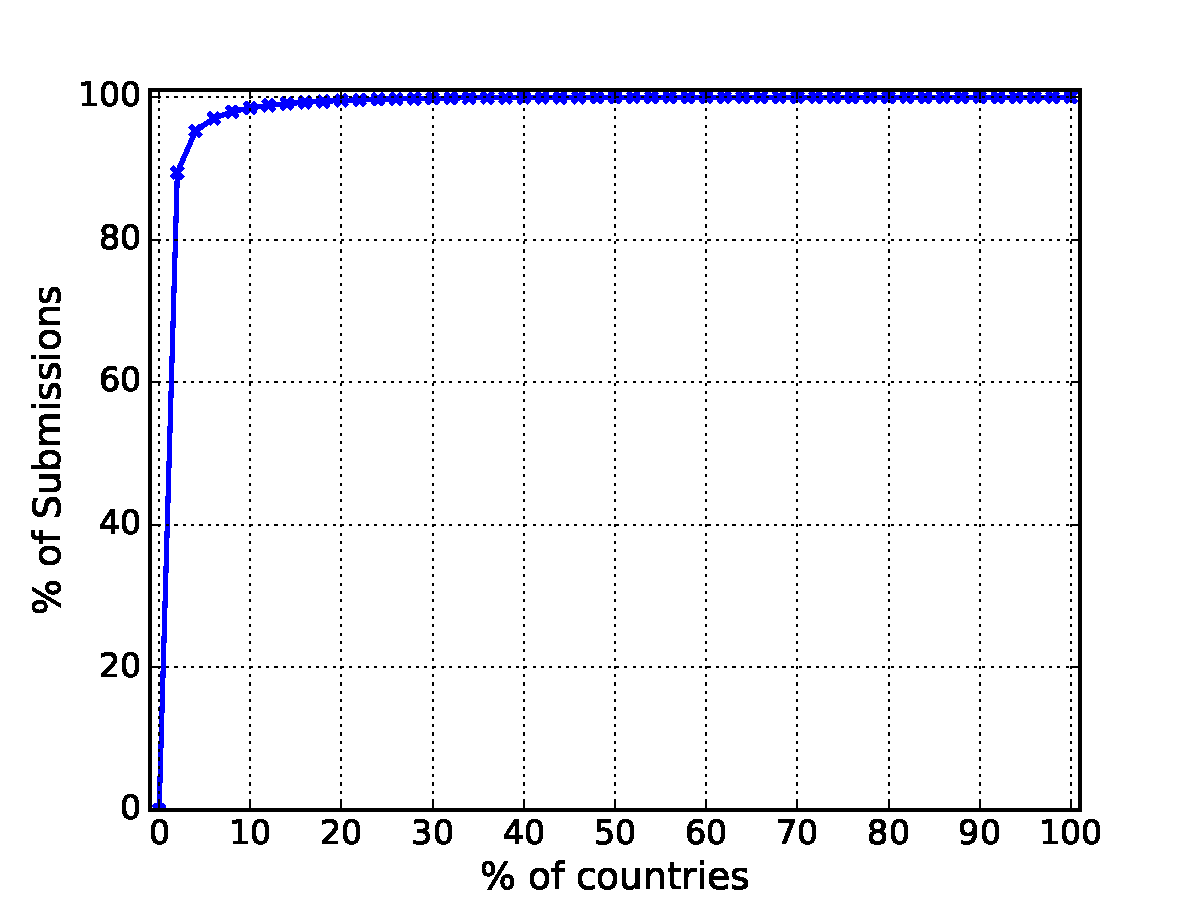
\includegraphics[width=2.5in]{figure/country}
\mycaption{fig:country}{Skewness of malware submissions from different countries in November 2015.}
{Accumulation distribution of malwares submitted from different countries in November 2015.}
%\label{fig:acum}
\end{center}
\vspace{-0.25in}
\end{figure}

There are also around 0.6 million malwares, 
whose submission countries VirusTotal fails to provide. 
All other malwares are submitted from 164 distinct countries. 
The top 5 countries are Canada, USA, China, France, and Germany. 
As shown in Figure~\ref{fig:country}, 
malware submissions are also distributed unbalanced among different countries. 

{\bf When?} How life-time distributes for malwares submitted to VirusTotal? 
Specifically, how long is it between submission time and when malwares firstly seen on VirusTotal?

\begin{figure}[t!]
\begin{center}
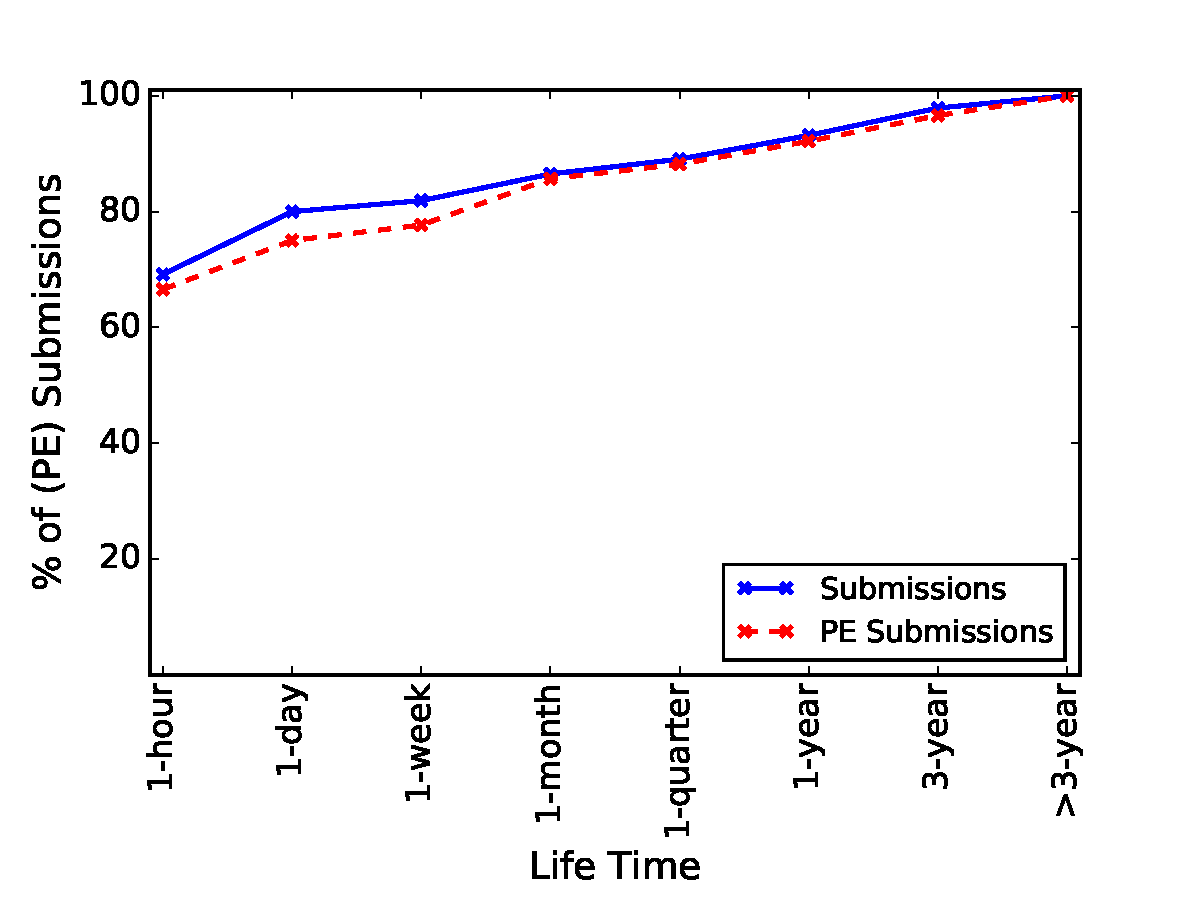
\includegraphics[width=2.5in]{figure/lifetime}
\mycaption{fig:life}{Malwares' lifetime in November 2015.}
{Accumulation distribution of malwares' lifetime in November 2015.}
%\label{fig:acum}
\end{center}
\vspace{-0.25in}
\end{figure}

As shown in Figure~\ref{fig:life}, malwares submitted to VirusTotal are quite new. 
More than 75\% malware submissions are firstly seen on VirusTotal.
For more than 90\% malware submissions, 
their submission time is less than one month since it was firstly seen on VirusTotal.  